\newprob{1715746137}
{
    以下哪些關於熱的陳述是正確的?
    % \par Which of the following statements about heat is/ are true?
    \begin{enumerate}[label=\sd]
        \item 熱是用來描述兩個物體之間由於溫度差而轉移的能量。
              %   \par Heat is used to describe the energy transferred from one body to another as a result of a temperature difference between them.
        \item 熱是用來描述構成物體的所有粒子的總動能。
              %   \par Heat is used to describe the total kinetic energy of all the particles making up the body.
        \item 當熱供應給一個物體時,其內能必定增加。
              %   \par When heat is supplied to a body, its internal energy must increase.
    \end{enumerate}
    \begin{choices}
        \choice 只有(1)
        \choice 只有(3)
        \CorrectChoice 只有(1)和(3)
        \choice 只有(2)和(3)
    \end{choices}
}{}

\newprob{1715747886}
{
    P和Q是由相同金屬製成的兩個立方體。 P的邊長是Q的兩倍。最初P的溫度較高。如下圖所示,它們互相接觸。所有外露表面均與周圍隔離。
    % \par P and Q are two cubes made of the same metal. The length of Pis double that of Q. Initially P is at a higher temperature. They are put in contact with each other as shown below. All exposed surfaces are insulated from the surroundings.
    \begin{figure}[h]
        \centering
        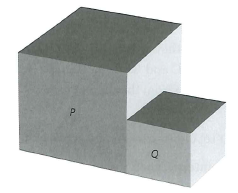
\includegraphics[width=0.4\linewidth]{assets/MCQ2.png}
    \end{figure}
    \par 達到熱平衡後,以下哪些陳述是正確的?
    % \par After thermal equilibrium is reached, which of the following statements are correct?
    \medskip
    \begin{enumerate}[label=\sd]
        \item P和Q的粒子的平均動能相同。
              %   \par The average kinetic energy of the particles of P and Q are the same.
        \item P和Q的粒子的平均勢能相同。
              %   \par The average potential energy of the particles of P and Q are the same.
        \item P的內能是Q的四倍。
              %   \par The internal energy of P is four times as large as that of Q.
    \end{enumerate}
    \begin{choices}
        \CorrectChoice 只有(1)和(2)
        \choice 只有(1)和(3)
        \choice 只有(2)和(3)
        \choice (1), (2) 和 (3)
    \end{choices}
}{}

\newprob{1715747911}
{
    以下哪些關於熱的陳述是正確的?
    % \par Which of the following statements about heat is/are true?
    \medskip
    \begin{enumerate}[label=\sd]
        \item 熱必定是從高溫物體流向低溫物體。
              %   \par Heat is used to describe the energy transferred from one body to another as a result of a temperature difference between them.
        \item 熱必定是從內能較高的物體流向內能較低的物體。
              %   \par Heat is used to describe the total kinetic energy of all the particles making up the body.
        \item 當熱供應給固體物體時,固體粒子振動所造成的平均速率會增加。
              %   \par When heat is supplied to a solid body, the particles of the solid vibrate with greater average speed.
    \end{enumerate}\medskip
    \begin{choices}
        \choice 只有(1)
        \choice 只有(3)
        \CorrectChoice 只有(1)和(3)
        \choice 只有(2) 和 (3)
    \end{choices}
}{}

\newprob{1715747994}
{
    下表給出了兩種液體P和Q的一些數據。以下哪些敘述是正確的?
    % \par Some data of two liquids P and Q are given in the table below. Which of the following statements is / are correct.
    \begin{table}[h]
        \begin{center}
            \begin{tabular}{|c|c|c|}
                \hline
                                            & 液體liquid P  & 液體liquid Q  \\
                \hline
                質量 mass                     & \qty{1}{kg} & \qty{3}{kg} \\
                \hline
                比熱容量 specific heat capacity & \shc{3900}  & \shc{1300}  \\
                \hline
                溫度 temperature              & \oc{60}     & \oc{20}     \\
                \hline
                沸點 boiling point            & \oc{120}    & \oc{80}     \\
                \hline
            \end{tabular}
        \end{center}
    \end{table}
    \begin{enumerate}[label=\sd]
        \item 液體P的內能必須大於液體Q的內能。
              %   \par The internal energy of P must be larger than that of Q.
        \item 它們具有相同的熱容量。
              %   \par They have the same heat capacity.
        \item 如果以相同的速率向兩種液體供熱,液體Q將首先開始沸騰。
              %   \par If heat is supplied to the two liquids at the same rate, liquid Q will start to boil first.
    \end{enumerate}
    % \clearpage
    \begin{choices}
        \choice 只有(1)
        \CorrectChoice 只有(2)
        \choice 只有(3)
        \choice (1), (2) 和 (3)
    \end{choices}

}{}

\newprob{1715748077}
{
    休息時,一個人的新陳代謝率約為\qty{120}{J.s^{-1}}。這種能量以熱的形式從身體流出。假設當人進入浴缸時,裡面裝有\qty{200}{kg}的水,最初溫度為\oc{27}。如果人體產生的熱量只轉移到水中,請估計1小時後水的溫度。
    \par 已知:水的比熱容量=\shc{4200}。
    % \par When resting, a person has a metabolic rate of about \qty{120}{J.s^{-1}}. This energy flows out of the body as heat. Suppose the person is immersed in a tub containing \qty{200}{kg} of water, initially at \oc{27} when the person gets into the tub. If the heat generated in the person goes into water only, estimate the temperature of the water after 1 hour.
    % \par Given: specific heat capacity of water = \shc{4200}.
    \begin{choices}
        \CorrectChoice \oc{27.5}
        \choice \oc{30}
        \choice \oc{32}
        \choice \oc{33}
    \end{choices}
}{}

\newprob{1715748155}
{
    在一個熱容量為\hc{20}的容器中,一個功率為\qty{100}{W}的浸入式加熱器加熱\qty{1.5}{kg}的液體X,時間為7.5分鐘。液體X的溫度從\oc{20}升高到\oc{30},並且有\qty{600}{J}的能量散失到周圍環境中。計算液體X的比熱容量。
    % \qty{1.5}{kg} of liquid X is heated up by an immersion heater of power \qty{100}{W} for 7.5 minutes in a vessel of heat capacity \hc{20} . The temperature of Xis raised from \oc{20} to \oc{30} and \qty{600}{J} of energy is lost to the surroundings. Calculate the specific heat capacity of liquid X.
    \begin{choices}
        \choice \shc{5900}
        \choice \shc{4425}
        \choice \shc{3000}
        \CorrectChoice \shc{2950}
    \end{choices}
}{}

\newprob{1715748162}
{
    以下哪項陳述可以用水的高比熱容量來解釋?
    % \par Which of the following can be explained by the high specific heat capacity of water?
    \begin{enumerate}[label=\sd]
        \item 在夏天,一碗熱粥要很長時間才能冷卻下來。
              %   \par In summer it takes a long time for a bowl of hot congee to cool down.
        \item 在冬天,一個人走出房子外面,身體溫度不會很快下降。
              %   \par When a man walks outside a house in cold winter, his body temperature will not drop quickly.
        \item 汽車炎熱的引擎使用水來作冷卻劑。
              %   \par In radiator, water is used as coolant for hot car engines.
    \end{enumerate}
    \begin{choices}
        \choice 只有(1)
        \choice 只有(1)和(2)
        \choice 只有(1)和(3)
        \CorrectChoice (1), (2) 和 (3)
    \end{choices}
}{}

\newprob{1715748305}
{
    兩種液體X和Y在相同的容器中被相同功率的加熱器分別加熱,容器的熱容量可以忽略不計。根據圖表,時間和溫度的變化關係如下。X的質量是Y的兩倍。以下哪些說法是正確的?
    % \par Two liquids X and Y are heated separately in identical containers of negligible heat capacity by heaters of the same power output. The temperature variation with time is shown in the graph. Mass of X is double that of Y. Which of the following statements are correct?
    \begin{figure}[h]
        \centering
        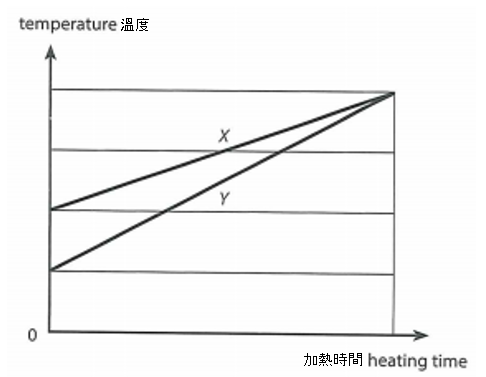
\includegraphics[width=0.5\linewidth]{assets/16.png}
    \end{figure}
    \begin{enumerate}[label=\sd]
        \item 加熱過程中沒有熱量散失到周圍環境。
              %   \par There is no heat lost to the surroundings during the heating process.
        \item $c_x: c_y=3:4$,其中$c_x$和$c_y$分別是X和Y的比熱容量。
              %   \par $c_x: c_y=3:4$, where $c_x$ and $c_y$ are the specific heat capacities of X and Y respectively.
        \item X的熱容量: Y的熱容量= $3:2$
              %   \par Heat capacity of X: heat capacity of Y = $3 : 2$.
    \end{enumerate}
    % \clearpage
    \begin{choices}
        \choice 只有(1)和(2)
        \choice 只有(1)和(3)
        \choice 只有(2)和(3)
        \CorrectChoice (1), (2) 和 (3)
    \end{choices}
}{}

\newprob{1715748346}
{
    杰克想準備一些奶茶。他將\qty{50}{g}溫度為\oc{15}的牛奶倒入一個杯子裡,裡面有\qty{200}{g}溫度為\oc{80}的茶。估計奶茶的溫度。
    % \par Jack wants to prepare some milk tea. He pours \qty{50}{g} of milk at \oc{15} into a cup containing \qty{200}{g} of tea at \oc{80}. Estimate the temperature of the milk tea.
    \par 杯子的熱容量 = \hc{100}
    \par 牛奶的比熱容量 = \shc{3500}
    \par 茶的比熱容量  = \shc{4200}

    \begin{choices}
        \choice \oc{64}
        \choice \oc{66}
        \choice \oc{68}
        \CorrectChoice \oc{70}
    \end{choices}
}{}

\newprob{1715748387}
{
    兩個由相同金屬製成的方塊X和Y。 X塊比Y塊大。如圖所示,X和Y的初始溫度分別為\oc{20}和\oc{80}。將它們放在一起,所有外露表面均與周圍隔熱。以下哪些陳述是正確的?
    % \par Two blocks X and Y are made of the same metal. Block X is larger than block Y. The initial temperatures of X and Y are \oc{20} and \oc{80} as shown. They are placed in contact and all exposed surfaces are well insulated from the surroundings. Which of the following statements are correct?
    \begin{figure}[h]
        \centering
        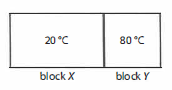
\includegraphics[width=0.35\linewidth]{assets/Screenshot 2023-08-29 143228.png}
    \end{figure}
    \begin{enumerate}[label=\sd]
        \item 熱從Y流向X,直到達到熱平衡狀態。
              %   \par Heat flows from Y to X until steady state is reached.
        \item 在熱平衡時,X塊的內能必須高於Y塊的內能。
              %   \par At steady state the internal energy ofblockXmust be higher than that of block Y.
        \item 最終的穩定溫度低於\oc{50}。
              %   \par The final steady temperature is lower than \oc{50}.
    \end{enumerate}
    \begin{choices}
        \choice 只有(1)和(2)
        \choice 只有(1)和(3)
        \choice 只有(2)和(3)
        \CorrectChoice (1), (2) 和 (3)
    \end{choices}
}{}

\newprob{1715748428}
{
    一種合金由兩種金屬P和Q按質量比$3:2$組成。P和Q的比熱容量分別為\shc{300}和\shc{950}。一個質量為\qty{4}{kg}的容器是由這種合金製成的。這個容器的熱容量是多少?
    % \par An alloy is composed of two metals P and Q in the ratio $3 : 2$ by mass. The specific heat capacities of P and Q are \shc{300} and \shc{950} respectively. A container of mass \qty{4}{kg} is made from this alloy. What is heat capacity of this container?
    \begin{choices}
        \choice \hc{560}
        \choice \hc{625}
        \choice \hc{1250}
        \CorrectChoice \hc{2240}
    \end{choices}
}{}

\newprob{1715748440}
{
    一個大碗P裝有\oc{70}的熱水,另一個小碗Q裝有\oc{35}的水。熱水和冷水的體積比為$3:2$。將Q中的水倒入P中,並充分攪拌。假設沒有熱量損失,混合後的水的預期溫度是多少?(忽略碗P的熱容量)
    % A large bowl P contains hot water at 70 °C and another smaller bowl Q contains water at \oc{35}. The volumes of hot water to cold water are in the ratio $3 : 2$. Water from Q is poured into P and stirred thoroughly. What is the expected temperature of the water after mixing, assuming no loss of heat? (Neglect the heat capacity of bowl P.)
    \begin{choices}
        \choice \oc{40}
        \choice \oc{44}
        \choice \oc{48}
        \CorrectChoice \oc{56}
    \end{choices}
}{}

\newprob{1715748450}
{
    一個海灘派對上的冰箱裡有12罐飲料。所有的冰都融化了,冰箱裡有\qty{2}{kg}的水。水和飲料的溫度是\oc{5}。每個罐子裡有\qty{0.35}{kg}的飲料,比熱容量為\shc{3800}。罐子的熱容量可以忽略不計。有人把一個\qty{6.5}{kg}、溫度為\oc{30}的西瓜加到冰箱裡。請計算飲料和西瓜的最終溫度。忽略冰箱的熱容量,並假設沒有吸收來自周圍環境的熱量。(取西瓜的比熱容量為\shc{4200})
    % \par An ice chest at a beach party contains 12 cans of soft drinks. All the ice has melted and the chest contains \qty{2}{kg} of water. The temperature of the water and the soft drinks is \oc{5}. Each can contains \qty{0.35}{kg} of soft drink, of specific heat capacity \shc{3800}. The heat capacity of the can is negligible. Someone adds a \qty{6.5}{kg} watermelon at \oc{30} to the chest. Calculate the final temperature of the drinks and watermelon. Neglect the heat capacity of the chest and assume there is no heat absorbed from the surroundings. (Take the specific heat capacity of watermelon to be \shc{4200})
    \begin{choices}
        \choice \oc{17.8}
        \CorrectChoice \oc{18.2}
        \choice \oc{20.8}
        \choice \oc{22.6}
    \end{choices}
}{}